\documentclass[tikz,border=5pt]{standalone}
\usepackage{tikz}
\usetikzlibrary{calc,angles,quotes}

\begin{document}
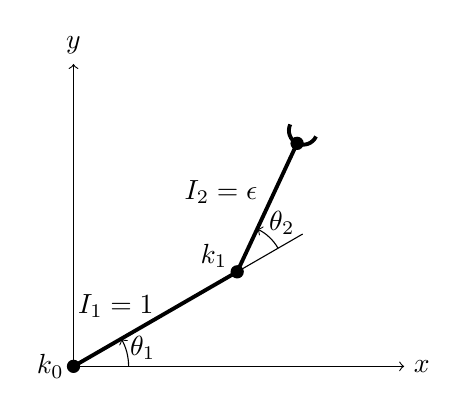
\begin{tikzpicture}[scale=1.2]

  % Parameters
  \def\lone{2}          % l1
  \def\ltwo{1.5}        % l2
  \def\thetaone{30}     % theta1 in degrees
  \def\thetatwo{65}     % theta2 in degrees

  \def\armthick{1.4pt}  % thickness for main arm segments and pincer

  % Mass positions:
  \coordinate (m0) at (0,0); % m0 at origin

  % m1 at p1 = l1 (cos theta1, sin theta1)
  \coordinate (m1) at ({\lone*cos(\thetaone)},{\lone*sin(\thetaone)});

  % m2 at p2 = p1 + l2 (cos theta2, sin theta2)
  \coordinate (m2) at ({\lone*cos(\thetaone)+\ltwo*cos(\thetatwo)},
                       {\lone*sin(\thetaone)+\ltwo*sin(\thetatwo)});

  % For the x-axis reference direction
  \coordinate (xpos) at (1,0);

  % Total radius to size axes
  \pgfmathsetmacro{\Xaxis}{\lone+\ltwo+0.0}
  \pgfmathsetmacro{\Yaxis}{\lone+\ltwo-0.3}

  % Axes from m0 (origin)
  \draw[->] (0,0) -- (\Xaxis,0) node[right] {$x$};
  \draw[->] (0,0) -- (0,\Yaxis) node[above] {$y$};

  % Extended "robot arms"
  % Extend line m0--m1 a bit further to meet the theta_2 arc
  \coordinate (m1ext) at ($(m0)!1.4!(m1)$); % extension beyond m1
  \draw (m0) -- (m1ext);  % extension stays thin

  % Extend line m1--m2 slightly beyond m2
  \coordinate (m2ext) at ($(m1)!1.0!(m2)$);
  \draw (m1) -- (m2ext);  % extension stays thin

  % Main arm segments (THICK)
  \draw[line width=\armthick] (m0) -- (m1);
  \draw[line width=\armthick] (m1) -- (m2);

  % Label for l1
  \path (m0) -- (m1) node[midway, above left=-1mm] {$I_1 = 1$};

  % Label for l2
  \path (m1) -- (m2) node[midway, left, yshift=2mm] {$I_2 = \epsilon$};


  % Draw masses
  \fill (m0) circle (2pt);
  \fill (m1) circle (2pt);
  \fill (m2) circle (2pt);

  % Labels for masses
  \node[left]  at (m0) {$k_0$};
  \node[left, yshift=2mm]  at (m1) {$k_1$};
  %\node[below right] at (m2) {$m_2$};

  % Angle theta1 between x-axis and segment m0--m1
  \pic[
    draw,
    ->,
    "$\theta_1$",
    angle eccentricity=1.3,
    angle radius=0.7cm
  ] {angle = xpos--m0--m1};

  % Angle theta2 between extension of m0--m1 and m1--m2
  \pic[
    draw,
    ->,
    "$\theta_2$",
    angle eccentricity=1.4,
    angle radius=0.6cm
  ] {angle = m1ext--m1--m2};

  % Robot pincer at m2:
  % Center lies along line m1--m2 beyond m2
  \coordinate (pincerC) at ($(m1)!1.1!(m2)$);

  % Draw semicircular pincer (THICK)
  \draw[line width=\armthick]
    let
      \p1 = (pincerC),
      \p2 = (m2),
      \n1 = {atan2(\y2-\y1,\x2-\x1)},      % angle from center to m2
      \n2 = {veclen(\x2-\x1,\y2-\y1)}      % radius = |C m2|
    in
      (pincerC) ++(\n1-90:\n2)
        arc[start angle=\n1-90, end angle=\n1+90, radius=\n2];

\end{tikzpicture}
\end{document}

